% VLDB template version of 2020-03-05 enhances the ACM template, version 1.7.0:
% https://www.acm.org/publications/proceedings-template
% The ACM Latex guide provides further information about the ACM template

\documentclass{article}
\usepackage{listings}
\usepackage[margin=20mm]{geometry}
\usepackage{graphicx}
\usepackage{amsfonts}
\usepackage{amsmath}
\usepackage{physics}
\usepackage{parskip}
\usepackage{enumitem}
\usepackage{cancel}

%% The following content must be adapted for the final version
% paper-specific
\newcommand\vldbdoi{XX.XX/XXX.XX}
\newcommand\vldbpages{XXX-XXX}
% issue-specific
\newcommand\vldbvolume{14}
\newcommand\vldbissue{1}
\newcommand\vldbyear{2020}
% should be fine as it is
\newcommand\vldbauthors{\authors}
\newcommand\vldbtitle{\shorttitle} 
% leave empty if no availability url should be set
\newcommand\vldbavailabilityurl{http://vldb.org/pvldb/format_vol14.html}

\newcommand\oname\operatorname

\newtheorem{theorem}{Teor.}
\newtheorem{definition}{Def.}
\newtheorem{example}{Ej.}
\newtheorem{excercise}{Ejer.}

\begin{document}

% Note to self:
%   "It is never possible to expose anyone to both treatments, and therefore statistical inference would still be needed to asses the \textit{causal inference}.

\textbf{Ex. 1.12.1: }Conditional probability: suppose that if $\theta=1$, then $y$ has a normal distribution with mean $1$ and standard deviation $\sigma$, and if $\theta=2$, then $y$ has a normal distribution with mean $2$ and standard deviation $\sigma$. Also, suppose $\oname{Pr}(\theta=1)=0.5$ and $\oname{Pr}(\theta=2)=0.5$.

\begin{enumerate}[label=\alph*]
	\item For $\theta=2$, write the formula for the marginal probability density for $y$ and sketch it.
	\item What is $\oname{Pr}(\theta=1|y=1)$, again supposing $\sigma=2$?
	\item Describe how the posterior density of $\theta$ changes in shape as $\sigma$ is increased and as it is decreased.
\end{enumerate}

\textbf{Answer:}

The formula for the marginal probability is that of $\mathcal N(\theta,\,\sigma^2)$:
\begin{align*}
	p(y|\theta=2)&=\frac1{\sqrt{2\pi\sigma^2}}\exp\left(-\frac12\left(\frac{x-2}\sigma\right)^2\right).
\end{align*}

As for the sketch, I'm too lazy to do it. It's a bell shape, centered at $2$ and $\sigma$ being half the width at about $0.61$ height. There's an xkcd-looking MatPlotLib plot in Figure \ref{fig:1.12.1}.
\begin{figure}[h]
	\centering
	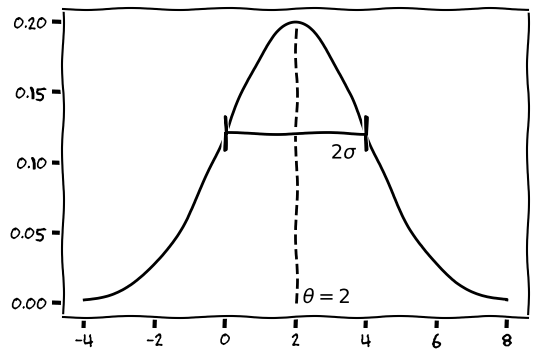
\includegraphics[width=0.4\textwidth]{Numerical/1.12.1}
	\caption{Your typical bell thingy with $\sigma=2$ and mean $2$}
	\label{fig:1.12.1}
\end{figure}

Now then,
\begin{align*}
	\oname{Pr}(\theta=1|y=1)&=\frac{\oname{Pr}(\theta=1)\oname{Pr}(y=1|\theta=1)}{\oname{Pr}(\theta=1)\oname{Pr}(y=1|\theta=1)+\oname{Pr}(\theta=2)\oname{Pr}(y=2|\theta=2)}\\
	&=\frac{0.5\cdot\frac1{\sqrt{8\pi}}}{0.5\cdot\frac1{\sqrt{8\pi}}+0.5\cdot\frac1{\sqrt{8\pi}}\exp\left(-\frac18\right)}\\
	&\approx0.53.
\end{align*}

The posterior for $\theta$ gets more homogeneous as $\sigma$ increases, and instead gets closer to $(1, 0)$ otherwise, since $\sigma$ directly defines the overlap between both likelihood functions as functions of $y$.

\textbf{Ex. 1.12.2: }Conditional means and variances: show that $(1.8)$ and $(1.9)$ hold if $u$ is a vector.

\textbf{Answer:}

No, $u$ are a vector.

Just kidding. Proof of $(1.8)$ is symbolically the same. As to $(1.9)$, it is \textit{about} the same. First, note that
\begin{align*}
	\oname{var}(x)&=\mathrm E\left[\left(x-\mathrm E(x)\right)\left(x-\mathrm E(x)\right)^T\right]\\
	&=\mathrm E\left[\left(x-\mathrm E(x)\right)\left(x^T-\left(\mathrm E(x)\right)^T\right)\right]\\
	&=\mathrm E\left[xx^T-x\left(\mathrm E(x)\right)^T-\mathrm E(x)x^T+\left(\mathrm E(x)\right)\left(\mathrm E(x)\right)^T\right]\\
	&=\mathrm E\left(xx^T\right)-\left(\mathrm E(x)\right)\left(\mathrm E(x)\right)^T.
\end{align*}
The result then follows replacing any occurrence of $x^2$ by $xx^T$.

\textbf{Ex. 1.12.3: }Probability calculation for genetics (from Lindley, 1965): suppose that in each individual of a large population there is a pair of genes, each of which can be either $x$ or $X$, that controls eye color: those with $xx$ have blue eyes, while heterozygotes (those with $Xx$ or $xX$) and those with $XX$ have brown eyes. The proportion of blue-eyed individuals is $p^2$ and of heterozygotes is $2p(1-p)$, where $0<p<1$. Each parent transmits one of its own genes to the child; if a parent is a heterozygote, the probability that it transmits the gene of type $X$ is $\frac12$. Assuming random mating, show that among brown-eyed children of brown-eyed parents, the expected proportion of heterozygotes is $2p/(1+2p)$. Suppose Judy, a brown-eyed child of brown-eyed parents, marries a heterozygote, and they have $n$ children, all brown-eyed. Find the posterior probability that Judy is a heterozygote and the probability that her first grandchild has blue eyes.

\textbf{Answer:}

Denoting $p_1$ and $p_2$ both parents' alleles, random mating implies $p(p_1|p_2)$ and $p(p_2)$ are both given by the population's proportion of people with $p_2$ and $p_1$ after $p_2$. We'll also use the hypothesis of a large pool of people, so that $p$ remains approximately equal after picking one of the parents. We thus have $p(p_1,\,p_2)=p(p_1)\,p(p_2)$.

So, if both parents are brown-eyed, they're one from $\{xX,\,Xx,\,XX\}$. The conditional probability of being any of the first two is
\begin{align*}
	\oname{Pr}(xX+Xx|xX+Xx+XX)&=\frac{\oname{Pr}((xX+Xx)(xX+Xx+XX))}{\oname{Pr}(xX+Xx+XX)}\\
	&=\frac{2p(p-1)}{2p(p-1)+(1-p)^2}\\
	&=\frac{2p}{1+p}.
\end{align*}
And the probability of transmiting either allele is then $1/2$. The probability of being an heterocygote is twice the probability that one of the parent gives $x$ and the other $X$, so
\begin{align*}
	&2\left(\frac12\frac{2p}{1+p}\right)\left(\frac12\frac{2p}{1+p}+\frac{1-p}{1+p}\right)\\
	&2\left(\frac12\frac{2p}{1+p}\right)\left(\frac1{1+p}\right)\\
	&\frac{2p}{(1+p)^2}.
\end{align*}
Finally, since we want this conditioned to the fact that they're all brown eyed, we must quotient this with the probability of being brown eyed, which is the above quantity plus the probability that both parents give $X$, $1/(1+p)^2$, so the final proportion is
\begin{align*}
	&\left[\frac{2p}{(1+p)^2}\right]\left[\frac{2p}{(1+p)^2}+\frac1{(1+p)^2}\right]^{-1}\\
	&=\frac{2p}{2p+1}.
\end{align*}

We are now asked the posterior probability of Judy being heterozygote after blah blah blah. So the priors of them being and not being heterozygote are $2p/(2p+1)$ and $1/(2p+1)$. The likelihood of the $n$ childrens are $\left(\frac34\right)^n$ and $1$ respectively, so that the posterior probability is
\begin{align*}
	\frac{2p}{2p+\left(\frac43\right)^n},
\end{align*}
which of course tends to $0$ as $n$ increases, since the likelihood of not having a blue eyed child decreases as $n$ increases.

\textbf{Ex. 1.12.4: }Probability assignment: we will use the football dataset to estimate some conditional probabilities about professional football games. There were twelve games with point spread of $8$ points; the outcomes in those games were: $-7$, $-5$, $-3$, $-3$, $1$, $6$, $7$, $13$, $15$, $16$, $20$, and $21$, with positive values indicating wins by the favorite and negative values indicating wins by the underdog. Consider the following conditional probabilities:
\begin{align*}
	&\oname{Pr}(\text{favorite wins}|\text{point spread}=8),\\
	&\oname{Pr}(\text{favorite wins by at least $8$}|\text{point spread}=8),\\
	&\oname{Pr}(\text{favorite wins by at least $8$}|\text{point spread}=8\text{ and favorite wins}).
\end{align*}
\begin{enumerate}[label=\alph*]
	\item Estimate each of these using the relative frequencies of games with a point spread of $8$.
	\item Estimate each using the normal approximation for the distribution of $(\text{outcome}-\text{point spread})$.
\end{enumerate}

\textbf{Answer: }

Point a is just counting:
\begin{align*}
	&\oname{Pr}(\text{favorite wins}|\text{point spread}=8)=8/12\approx0.58\\
	&\oname{Pr}(\text{favorite wins by at least $8$}|\text{point spread}=8)=5/12\approx0.42,\\
	&\oname{Pr}(\text{favorite wins by at least $8$}|\text{point spread}=8\text{ and favorite wins})=5/8\approx0.63.
\end{align*}

Point b uses the model $P(\text{wins by $\hat{y}$}|\text{point spread of $x$})=\mathcal N(\hat{y}|x,\,14^2)$, so
\begin{align*}
	\oname{Pr}(\text{favorite wins}|\text{point spread}=8)&=1-\Phi\left(\frac{0-8}{14}\right)\\
	&\approx0.72\\
	\oname{Pr}(\text{favorite wins by at least $8$}|\text{point spread}=8)&=0.5,\\
	\oname{Pr}(\text{favorite wins by at least $8$}|\text{point spread}=8\text{ and favorite wins})&\approx\frac{0.5}{0.72}\\
	&\approx0.69
\end{align*}

\textbf{Ex. 1.12.5: }Probability assignment: the $435$ U.S. Congressmembers are elected to two-year terms; the number of voters in an individual congressional election varies from $50\,000$ to $350\,000$. We will use various sources of information to estimate roughly the probability that at least one congressional election is tied in the next national election.
\begin{enumerate}[label=\alph*]
	\item Use any knowledge you have about U.S. politics. Specify clearly what information you are using to construct this conditional probability, even if your answer is just a guess.
	\item Use the following information: in the period $1900-1992$, there were $20\,597$ congressional elections, out of which $6$ were decided by fewer than $10$ votes and $49$ by fewer than $100$ votes.
\end{enumerate}

\textbf{Answer:}

Got no knowledge. Gonna skip this one.

\textbf{Ex. 1.12.6: }Conditional probability: approximately $1/125$ of all births are fraternal twins and $1/300$ of births are identical twins. Elvis Presley had a twin brother (who died at birth). What is the probability that Elvis was an identical twin? (You may approximate the probability of a boy or girl birth as $1/2$).

\textbf{Answer:}

We need
\begin{align*}
	P(\text{Identical}|\text{Both male})&=\frac{P(\text{Both male}|\text{Identical})P(\text{Identical})}{P(\text{Both male}|\text{Identical})P(\text{Identical})+P(\text{Both male}|\text{Fraternal})P(\text{Fraternal})}.
\end{align*}

This is pretty straightforward:
\begin{align*}
	P(\text{Both male}|\text{Identical})&=\frac12,\\
	P(\text{Identical})&=\frac1{300},\\
	P(\text{Both male}|\text{Fraternal})&=\frac12\frac12,\\
	P(\text{Fraternal})&=\frac1{125}
\end{align*}

It then follows that
\begin{align*}
	P(\text{Identical}|\text{Both male})&=5/11\approx0.45.
\end{align*}

\textbf{Ex. 1.12.7: }Conditional probability: the following problem is loosely based on the television game show \textit{Let's Make a Deal}. At the end of the show, a contestant is asked to choose one of three large boxes, where one box contains a fabulous prize and the other two boxes contain lesser prizes. After the contestant chooses a box, Monty Hall, the host of the show, opens one of the two boxes containing smaller prizes. (In order to keep the conclusion suspenseful, Monty does not open the box selected by the contestant.) Monty offers the contestant the opportunity to switch from the chosen box to the remaining unopened box. Should the contestant switch or stay with the original choice? Calculate the probability that the contestant wins under each strategy. This is an exercise in being clear about the information that should be conditioned on when constructing a probability judgement.

\textbf{Answer:}

Let $W_i=\text{the winning box is the $i$th}$, $P_i=\text{the player chose the $i$th box}$, $H_i=\text{the host opened the $i$th box}$. We then want
\begin{align*}
	P(W_1|P_2H_3)&=\frac{P(H_3|P_2W_1)P(W_1|P_2)}{P(H_3|P_2W_1)P(W_1|P_2)+P(H_3|P_2W_2)P(W_2|P_2)+P(H_3|P_2W_3)P(W_1|P_3)}\\
	&=\frac{1}{1+\frac12+0}\\
	&=\frac23.
\end{align*}

So, the obvious choice is to switch.

\textbf{Ex. 1.12.8: }Subjective probability: discuss the following statement. `The probability of event $E$ is considered ``subjective'' if two rational persons $A$ and $B$ can assign unequal probabilities to $E$, $P_A(E)$ and $P_B(E)$. These probabilities can also be interpreted as ``conditional'': $P_A(E)=P(E|I_A)$ and $P_B(E)=P(E|I_B)$, where $I_A$ and $I_B$ represent the knowledge available to persons $A$ and $B$, respectively'. Apply this idea to the following examples.
\begin{enumerate}[label=\alph*]
	\item The probability that a `$6$' appears when a fair die is rolled, where $A$ observes the outcome of the die roll and $B$ does not.
	\item The probability that Brazil wins the next World Cup, where $A$ is ignorant of soccer and $B$ is a knowledgeable sports fan.
\end{enumerate}

\textbf{Answer:}

I'd say both are subjective. The knowledge of the die throw \textit{before} observation is that there's $1/6$ probability for any side, since it's a fair die. But if $A$ knows the result of the die, then the probability distribution should no longer incorporate any uncertainty. The second example is more evident, since it is expected that people more knowledgeable have a better understanding of their degree of knowledge.

\textbf{Ex. 1.12.9: }Simulation of a queuing problem: a clinic has three doctors. Patients come into the clinic at random, starting at $9$ a.m., according to a Poisson process with time parameter $10$ minutes: that is, the time after opening at which the first patient appears follows an exponential distribution with expectation $10$ minutes and then, after each patient arrives, the waiting time until the next patient is independently exponentially distributed, also with expectation $10$ minutes. When a patient arrives, he or she waits until a doctor is available. The amount of time spent by each doctor with each patient is a random variable, uniformly distributed between $5$ and $20$ minutes. The office stops admitting new patients at $4$ p.m. and closes when the last patient is through with the doctor.
\begin{enumerate}[label=\alph*]
	\item Simulate this process once. How many patients came to the office? How many had to wait for a doctor? What was their average wait? When did the office close?
	\item Simulate the process $100$ times and estimate the median and $50\%$ interval for each of the summaries in $(a)$.
\end{enumerate}

\textbf{Answer:}

Script ``1.12.9.py'' generates these answers:
\input{Numerical/1.12.9.out}

The rest of answers can be found in Figure \ref{fig:1.12.9}.
\begin{figure}[h]
	\centering
	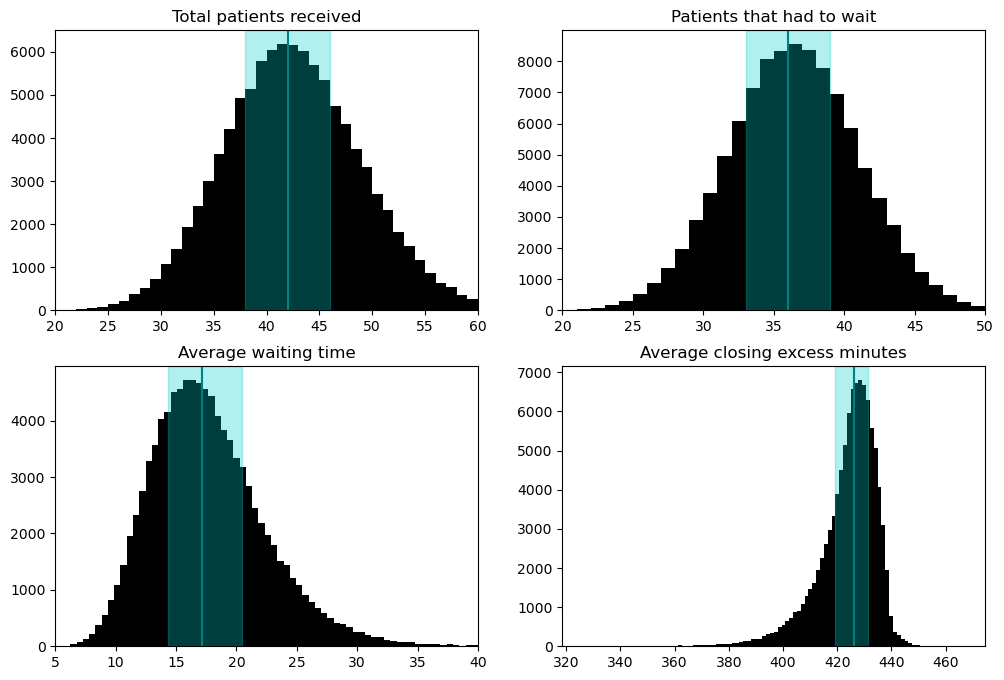
\includegraphics[width=0.8\textwidth]{Numerical/1.12.9}
	\caption{Histograms for the stuff after $100000$ runs.}
	\label{fig:1.12.9}
\end{figure}

\end{document}
\endinput
